% This file is generated by the MATLAB m-file laprint.m. It can be included
% into LaTeX documents using the packages graphicx, color and psfrag.
% It is accompanied by a postscript file. A sample LaTeX file is:
%    \documentclass{article}\usepackage{graphicx,color,psfrag}
%    \begin{document}% This file is generated by the MATLAB m-file laprint.m. It can be included
% into LaTeX documents using the packages graphicx, color and psfrag.
% It is accompanied by a postscript file. A sample LaTeX file is:
%    \documentclass{article}\usepackage{graphicx,color,psfrag}
%    \begin{document}% This file is generated by the MATLAB m-file laprint.m. It can be included
% into LaTeX documents using the packages graphicx, color and psfrag.
% It is accompanied by a postscript file. A sample LaTeX file is:
%    \documentclass{article}\usepackage{graphicx,color,psfrag}
%    \begin{document}% This file is generated by the MATLAB m-file laprint.m. It can be included
% into LaTeX documents using the packages graphicx, color and psfrag.
% It is accompanied by a postscript file. A sample LaTeX file is:
%    \documentclass{article}\usepackage{graphicx,color,psfrag}
%    \begin{document}\input{unnamed}\end{document}
% See http://www.mathworks.de/matlabcentral/fileexchange/loadFile.do?objectId=4638
% for recent versions of laprint.m.
%
% created by:           LaPrint version 3.16 (13.9.2004)
% created on:           28-Dec-2013 21:44:20
% eps bounding box:     15 cm x 9.4415 cm
% comment:              
%
\begin{psfrags}%
\psfragscanon%
%
% text strings:
\psfrag{s01}[][]{\color[rgb]{0,0,0}\setlength{\tabcolsep}{0pt}\begin{tabular}{c}-48787.0859\end{tabular}}%
\psfrag{s02}[][]{\color[rgb]{0,0,0}\setlength{\tabcolsep}{0pt}\begin{tabular}{c}-46015.0924\end{tabular}}%
\psfrag{s03}[][]{\color[rgb]{0,0,0}\setlength{\tabcolsep}{0pt}\begin{tabular}{c}-43243.0989\end{tabular}}%
\psfrag{s04}[][]{\color[rgb]{0,0,0}\setlength{\tabcolsep}{0pt}\begin{tabular}{c}-40471.1054\end{tabular}}%
\psfrag{s05}[][]{\color[rgb]{0,0,0}\setlength{\tabcolsep}{0pt}\begin{tabular}{c}-37699.1118\end{tabular}}%
\psfrag{s06}[][]{\color[rgb]{0,0,0}\setlength{\tabcolsep}{0pt}\begin{tabular}{c}-34927.1183\end{tabular}}%
\psfrag{s07}[][]{\color[rgb]{0,0,0}\setlength{\tabcolsep}{0pt}\begin{tabular}{c}-32155.1248\end{tabular}}%
\psfrag{s08}[][]{\color[rgb]{0,0,0}\setlength{\tabcolsep}{0pt}\begin{tabular}{c}-29383.1313\end{tabular}}%
\psfrag{s09}[][]{\color[rgb]{0,0,0}\setlength{\tabcolsep}{0pt}\begin{tabular}{c}-26611.1378\end{tabular}}%
\psfrag{s10}[][]{\color[rgb]{0,0,0}\setlength{\tabcolsep}{0pt}\begin{tabular}{c}-23839.1443\end{tabular}}%
\psfrag{s11}[][]{\color[rgb]{0,0,0}\setlength{\tabcolsep}{0pt}\begin{tabular}{c}-21067.1507\end{tabular}}%
\psfrag{s12}[][]{\color[rgb]{0,0,0}\setlength{\tabcolsep}{0pt}\begin{tabular}{c}-18295.1572\end{tabular}}%
\psfrag{s13}[][]{\color[rgb]{0,0,0}\setlength{\tabcolsep}{0pt}\begin{tabular}{c}-15523.1637\end{tabular}}%
\psfrag{s14}[][]{\color[rgb]{0,0,0}\setlength{\tabcolsep}{0pt}\begin{tabular}{c}-15523.1637\end{tabular}}%
\psfrag{s15}[][]{\color[rgb]{0,0,0}\setlength{\tabcolsep}{0pt}\begin{tabular}{c}-12751.1702\end{tabular}}%
\psfrag{s16}[][]{\color[rgb]{0,0,0}\setlength{\tabcolsep}{0pt}\begin{tabular}{c}-12751.1702\end{tabular}}%
\psfrag{s17}[][]{\color[rgb]{0,0,0}\setlength{\tabcolsep}{0pt}\begin{tabular}{c}-9979.17666\end{tabular}}%
\psfrag{s18}[][]{\color[rgb]{0,0,0}\setlength{\tabcolsep}{0pt}\begin{tabular}{c}-9979.17666\end{tabular}}%
\psfrag{s19}[][]{\color[rgb]{0,0,0}\setlength{\tabcolsep}{0pt}\begin{tabular}{c}-7207.18315\end{tabular}}%
\psfrag{s20}[][]{\color[rgb]{0,0,0}\setlength{\tabcolsep}{0pt}\begin{tabular}{c}-7207.18315\end{tabular}}%
\psfrag{s21}[][]{\color[rgb]{0,0,0}\setlength{\tabcolsep}{0pt}\begin{tabular}{c}-4435.18963\end{tabular}}%
\psfrag{s22}[][]{\color[rgb]{0,0,0}\setlength{\tabcolsep}{0pt}\begin{tabular}{c}-4435.18963\end{tabular}}%
\psfrag{s23}[][]{\color[rgb]{0,0,0}\setlength{\tabcolsep}{0pt}\begin{tabular}{c}-4435.18963\end{tabular}}%
\psfrag{s24}[][]{\color[rgb]{0,0,0}\setlength{\tabcolsep}{0pt}\begin{tabular}{c}-1663.19611\end{tabular}}%
\psfrag{s25}[][]{\color[rgb]{0,0,0}\setlength{\tabcolsep}{0pt}\begin{tabular}{c}-1663.19611\end{tabular}}%
\psfrag{s26}[][]{\color[rgb]{0,0,0}\setlength{\tabcolsep}{0pt}\begin{tabular}{c}-1663.19611\end{tabular}}%
\psfrag{s27}[][]{\color[rgb]{0,0,0}\setlength{\tabcolsep}{0pt}\begin{tabular}{c}-1663.19611\end{tabular}}%
\psfrag{s28}[][]{\color[rgb]{0,0,0}\setlength{\tabcolsep}{0pt}\begin{tabular}{c}1108.79741\end{tabular}}%
\psfrag{s29}[][]{\color[rgb]{0,0,0}\setlength{\tabcolsep}{0pt}\begin{tabular}{c}1108.79741\end{tabular}}%
\psfrag{s30}[][]{\color[rgb]{0,0,0}\setlength{\tabcolsep}{0pt}\begin{tabular}{c}1108.79741\end{tabular}}%
\psfrag{s31}[][]{\color[rgb]{0,0,0}\setlength{\tabcolsep}{0pt}\begin{tabular}{c}3880.79093\end{tabular}}%
\psfrag{s32}[][]{\color[rgb]{0,0,0}\setlength{\tabcolsep}{0pt}\begin{tabular}{c}3880.79093\end{tabular}}%
\psfrag{s33}[][]{\color[rgb]{0,0,0}\setlength{\tabcolsep}{0pt}\begin{tabular}{c}6652.78444\end{tabular}}%
\psfrag{s34}[][]{\color[rgb]{0,0,0}\setlength{\tabcolsep}{0pt}\begin{tabular}{c}6652.78444\end{tabular}}%
\psfrag{s35}[][]{\color[rgb]{0,0,0}\setlength{\tabcolsep}{0pt}\begin{tabular}{c}9424.77796\end{tabular}}%
\psfrag{s36}[][]{\color[rgb]{0,0,0}\setlength{\tabcolsep}{0pt}\begin{tabular}{c}12196.7715\end{tabular}}%
\psfrag{s37}[][]{\color[rgb]{0,0,0}\setlength{\tabcolsep}{0pt}\begin{tabular}{c}14968.765\end{tabular}}%
\psfrag{s38}[][]{\color[rgb]{0,0,0}\setlength{\tabcolsep}{0pt}\begin{tabular}{c}17740.7585\end{tabular}}%
\psfrag{s39}[][]{\color[rgb]{0,0,0}\setlength{\tabcolsep}{0pt}\begin{tabular}{c}20512.752\end{tabular}}%
\psfrag{s40}[][]{\color[rgb]{0,0,0}\setlength{\tabcolsep}{0pt}\begin{tabular}{c}23284.7456\end{tabular}}%
\psfrag{s41}[][]{\color[rgb]{0,0,0}\setlength{\tabcolsep}{0pt}\begin{tabular}{c}26056.7391\end{tabular}}%
\psfrag{s42}[][]{\color[rgb]{0,0,0}\setlength{\tabcolsep}{0pt}\begin{tabular}{c}28828.7326\end{tabular}}%
\psfrag{s43}[][]{\color[rgb]{0,0,0}\setlength{\tabcolsep}{0pt}\begin{tabular}{c}31600.7261\end{tabular}}%
\psfrag{s44}[t][t]{\color[rgb]{0,0,0}\setlength{\tabcolsep}{0pt}\begin{tabular}{c}x\end{tabular}}%
\psfrag{s45}[b][b]{\color[rgb]{0,0,0}\setlength{\tabcolsep}{0pt}\begin{tabular}{c}y\end{tabular}}%
\psfrag{s52}[lt][lt]{\color[rgb]{0,0,0}\setlength{\tabcolsep}{0pt}\begin{tabular}{l}g_1\end{tabular}}%
\psfrag{s53}[lt][lt]{\color[rgb]{0,0,0}\setlength{\tabcolsep}{0pt}\begin{tabular}{l}g_5\end{tabular}}%
\psfrag{s54}[lt][lt]{\color[rgb]{0,0,0}\setlength{\tabcolsep}{0pt}\begin{tabular}{l}f\end{tabular}}%
%
% Figure:
\resizebox{12cm}{!}{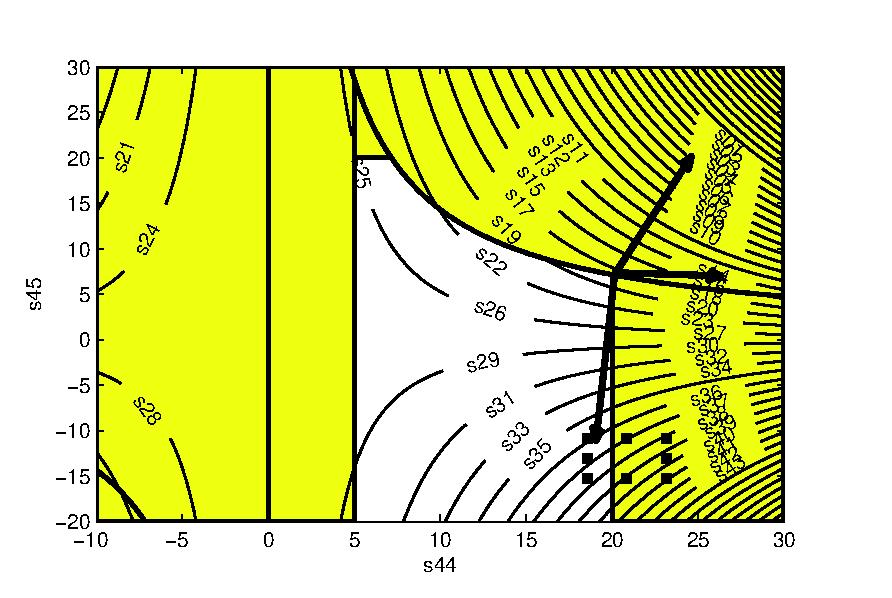
\includegraphics{unnamed.eps}}%
\end{psfrags}%
%
% End unnamed.tex
\end{document}
% See http://www.mathworks.de/matlabcentral/fileexchange/loadFile.do?objectId=4638
% for recent versions of laprint.m.
%
% created by:           LaPrint version 3.16 (13.9.2004)
% created on:           28-Dec-2013 21:44:20
% eps bounding box:     15 cm x 9.4415 cm
% comment:              
%
\begin{psfrags}%
\psfragscanon%
%
% text strings:
\psfrag{s01}[][]{\color[rgb]{0,0,0}\setlength{\tabcolsep}{0pt}\begin{tabular}{c}-48787.0859\end{tabular}}%
\psfrag{s02}[][]{\color[rgb]{0,0,0}\setlength{\tabcolsep}{0pt}\begin{tabular}{c}-46015.0924\end{tabular}}%
\psfrag{s03}[][]{\color[rgb]{0,0,0}\setlength{\tabcolsep}{0pt}\begin{tabular}{c}-43243.0989\end{tabular}}%
\psfrag{s04}[][]{\color[rgb]{0,0,0}\setlength{\tabcolsep}{0pt}\begin{tabular}{c}-40471.1054\end{tabular}}%
\psfrag{s05}[][]{\color[rgb]{0,0,0}\setlength{\tabcolsep}{0pt}\begin{tabular}{c}-37699.1118\end{tabular}}%
\psfrag{s06}[][]{\color[rgb]{0,0,0}\setlength{\tabcolsep}{0pt}\begin{tabular}{c}-34927.1183\end{tabular}}%
\psfrag{s07}[][]{\color[rgb]{0,0,0}\setlength{\tabcolsep}{0pt}\begin{tabular}{c}-32155.1248\end{tabular}}%
\psfrag{s08}[][]{\color[rgb]{0,0,0}\setlength{\tabcolsep}{0pt}\begin{tabular}{c}-29383.1313\end{tabular}}%
\psfrag{s09}[][]{\color[rgb]{0,0,0}\setlength{\tabcolsep}{0pt}\begin{tabular}{c}-26611.1378\end{tabular}}%
\psfrag{s10}[][]{\color[rgb]{0,0,0}\setlength{\tabcolsep}{0pt}\begin{tabular}{c}-23839.1443\end{tabular}}%
\psfrag{s11}[][]{\color[rgb]{0,0,0}\setlength{\tabcolsep}{0pt}\begin{tabular}{c}-21067.1507\end{tabular}}%
\psfrag{s12}[][]{\color[rgb]{0,0,0}\setlength{\tabcolsep}{0pt}\begin{tabular}{c}-18295.1572\end{tabular}}%
\psfrag{s13}[][]{\color[rgb]{0,0,0}\setlength{\tabcolsep}{0pt}\begin{tabular}{c}-15523.1637\end{tabular}}%
\psfrag{s14}[][]{\color[rgb]{0,0,0}\setlength{\tabcolsep}{0pt}\begin{tabular}{c}-15523.1637\end{tabular}}%
\psfrag{s15}[][]{\color[rgb]{0,0,0}\setlength{\tabcolsep}{0pt}\begin{tabular}{c}-12751.1702\end{tabular}}%
\psfrag{s16}[][]{\color[rgb]{0,0,0}\setlength{\tabcolsep}{0pt}\begin{tabular}{c}-12751.1702\end{tabular}}%
\psfrag{s17}[][]{\color[rgb]{0,0,0}\setlength{\tabcolsep}{0pt}\begin{tabular}{c}-9979.17666\end{tabular}}%
\psfrag{s18}[][]{\color[rgb]{0,0,0}\setlength{\tabcolsep}{0pt}\begin{tabular}{c}-9979.17666\end{tabular}}%
\psfrag{s19}[][]{\color[rgb]{0,0,0}\setlength{\tabcolsep}{0pt}\begin{tabular}{c}-7207.18315\end{tabular}}%
\psfrag{s20}[][]{\color[rgb]{0,0,0}\setlength{\tabcolsep}{0pt}\begin{tabular}{c}-7207.18315\end{tabular}}%
\psfrag{s21}[][]{\color[rgb]{0,0,0}\setlength{\tabcolsep}{0pt}\begin{tabular}{c}-4435.18963\end{tabular}}%
\psfrag{s22}[][]{\color[rgb]{0,0,0}\setlength{\tabcolsep}{0pt}\begin{tabular}{c}-4435.18963\end{tabular}}%
\psfrag{s23}[][]{\color[rgb]{0,0,0}\setlength{\tabcolsep}{0pt}\begin{tabular}{c}-4435.18963\end{tabular}}%
\psfrag{s24}[][]{\color[rgb]{0,0,0}\setlength{\tabcolsep}{0pt}\begin{tabular}{c}-1663.19611\end{tabular}}%
\psfrag{s25}[][]{\color[rgb]{0,0,0}\setlength{\tabcolsep}{0pt}\begin{tabular}{c}-1663.19611\end{tabular}}%
\psfrag{s26}[][]{\color[rgb]{0,0,0}\setlength{\tabcolsep}{0pt}\begin{tabular}{c}-1663.19611\end{tabular}}%
\psfrag{s27}[][]{\color[rgb]{0,0,0}\setlength{\tabcolsep}{0pt}\begin{tabular}{c}-1663.19611\end{tabular}}%
\psfrag{s28}[][]{\color[rgb]{0,0,0}\setlength{\tabcolsep}{0pt}\begin{tabular}{c}1108.79741\end{tabular}}%
\psfrag{s29}[][]{\color[rgb]{0,0,0}\setlength{\tabcolsep}{0pt}\begin{tabular}{c}1108.79741\end{tabular}}%
\psfrag{s30}[][]{\color[rgb]{0,0,0}\setlength{\tabcolsep}{0pt}\begin{tabular}{c}1108.79741\end{tabular}}%
\psfrag{s31}[][]{\color[rgb]{0,0,0}\setlength{\tabcolsep}{0pt}\begin{tabular}{c}3880.79093\end{tabular}}%
\psfrag{s32}[][]{\color[rgb]{0,0,0}\setlength{\tabcolsep}{0pt}\begin{tabular}{c}3880.79093\end{tabular}}%
\psfrag{s33}[][]{\color[rgb]{0,0,0}\setlength{\tabcolsep}{0pt}\begin{tabular}{c}6652.78444\end{tabular}}%
\psfrag{s34}[][]{\color[rgb]{0,0,0}\setlength{\tabcolsep}{0pt}\begin{tabular}{c}6652.78444\end{tabular}}%
\psfrag{s35}[][]{\color[rgb]{0,0,0}\setlength{\tabcolsep}{0pt}\begin{tabular}{c}9424.77796\end{tabular}}%
\psfrag{s36}[][]{\color[rgb]{0,0,0}\setlength{\tabcolsep}{0pt}\begin{tabular}{c}12196.7715\end{tabular}}%
\psfrag{s37}[][]{\color[rgb]{0,0,0}\setlength{\tabcolsep}{0pt}\begin{tabular}{c}14968.765\end{tabular}}%
\psfrag{s38}[][]{\color[rgb]{0,0,0}\setlength{\tabcolsep}{0pt}\begin{tabular}{c}17740.7585\end{tabular}}%
\psfrag{s39}[][]{\color[rgb]{0,0,0}\setlength{\tabcolsep}{0pt}\begin{tabular}{c}20512.752\end{tabular}}%
\psfrag{s40}[][]{\color[rgb]{0,0,0}\setlength{\tabcolsep}{0pt}\begin{tabular}{c}23284.7456\end{tabular}}%
\psfrag{s41}[][]{\color[rgb]{0,0,0}\setlength{\tabcolsep}{0pt}\begin{tabular}{c}26056.7391\end{tabular}}%
\psfrag{s42}[][]{\color[rgb]{0,0,0}\setlength{\tabcolsep}{0pt}\begin{tabular}{c}28828.7326\end{tabular}}%
\psfrag{s43}[][]{\color[rgb]{0,0,0}\setlength{\tabcolsep}{0pt}\begin{tabular}{c}31600.7261\end{tabular}}%
\psfrag{s44}[t][t]{\color[rgb]{0,0,0}\setlength{\tabcolsep}{0pt}\begin{tabular}{c}x\end{tabular}}%
\psfrag{s45}[b][b]{\color[rgb]{0,0,0}\setlength{\tabcolsep}{0pt}\begin{tabular}{c}y\end{tabular}}%
\psfrag{s52}[lt][lt]{\color[rgb]{0,0,0}\setlength{\tabcolsep}{0pt}\begin{tabular}{l}g_1\end{tabular}}%
\psfrag{s53}[lt][lt]{\color[rgb]{0,0,0}\setlength{\tabcolsep}{0pt}\begin{tabular}{l}g_5\end{tabular}}%
\psfrag{s54}[lt][lt]{\color[rgb]{0,0,0}\setlength{\tabcolsep}{0pt}\begin{tabular}{l}f\end{tabular}}%
%
% Figure:
\resizebox{12cm}{!}{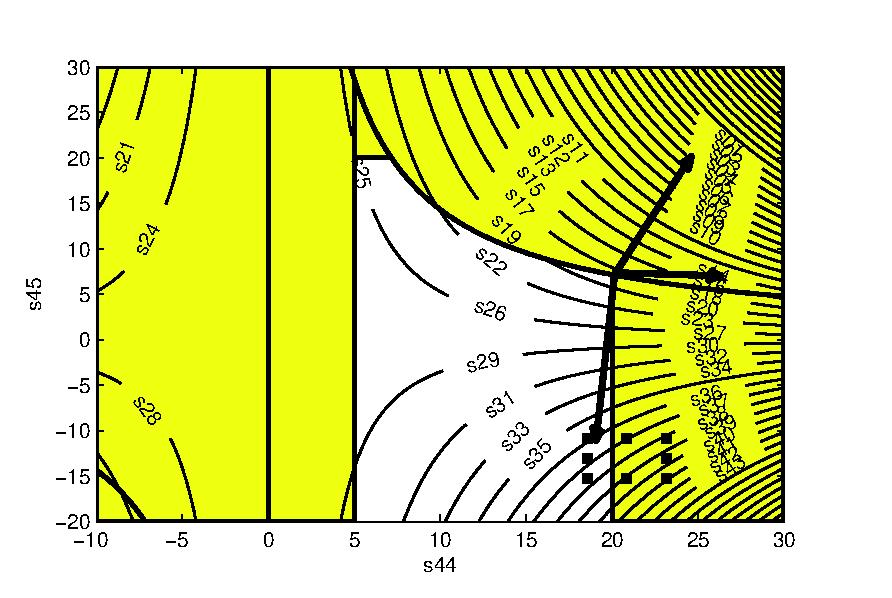
\includegraphics{unnamed.eps}}%
\end{psfrags}%
%
% End unnamed.tex
\end{document}
% See http://www.mathworks.de/matlabcentral/fileexchange/loadFile.do?objectId=4638
% for recent versions of laprint.m.
%
% created by:           LaPrint version 3.16 (13.9.2004)
% created on:           28-Dec-2013 21:44:20
% eps bounding box:     15 cm x 9.4415 cm
% comment:              
%
\begin{psfrags}%
\psfragscanon%
%
% text strings:
\psfrag{s01}[][]{\color[rgb]{0,0,0}\setlength{\tabcolsep}{0pt}\begin{tabular}{c}-48787.0859\end{tabular}}%
\psfrag{s02}[][]{\color[rgb]{0,0,0}\setlength{\tabcolsep}{0pt}\begin{tabular}{c}-46015.0924\end{tabular}}%
\psfrag{s03}[][]{\color[rgb]{0,0,0}\setlength{\tabcolsep}{0pt}\begin{tabular}{c}-43243.0989\end{tabular}}%
\psfrag{s04}[][]{\color[rgb]{0,0,0}\setlength{\tabcolsep}{0pt}\begin{tabular}{c}-40471.1054\end{tabular}}%
\psfrag{s05}[][]{\color[rgb]{0,0,0}\setlength{\tabcolsep}{0pt}\begin{tabular}{c}-37699.1118\end{tabular}}%
\psfrag{s06}[][]{\color[rgb]{0,0,0}\setlength{\tabcolsep}{0pt}\begin{tabular}{c}-34927.1183\end{tabular}}%
\psfrag{s07}[][]{\color[rgb]{0,0,0}\setlength{\tabcolsep}{0pt}\begin{tabular}{c}-32155.1248\end{tabular}}%
\psfrag{s08}[][]{\color[rgb]{0,0,0}\setlength{\tabcolsep}{0pt}\begin{tabular}{c}-29383.1313\end{tabular}}%
\psfrag{s09}[][]{\color[rgb]{0,0,0}\setlength{\tabcolsep}{0pt}\begin{tabular}{c}-26611.1378\end{tabular}}%
\psfrag{s10}[][]{\color[rgb]{0,0,0}\setlength{\tabcolsep}{0pt}\begin{tabular}{c}-23839.1443\end{tabular}}%
\psfrag{s11}[][]{\color[rgb]{0,0,0}\setlength{\tabcolsep}{0pt}\begin{tabular}{c}-21067.1507\end{tabular}}%
\psfrag{s12}[][]{\color[rgb]{0,0,0}\setlength{\tabcolsep}{0pt}\begin{tabular}{c}-18295.1572\end{tabular}}%
\psfrag{s13}[][]{\color[rgb]{0,0,0}\setlength{\tabcolsep}{0pt}\begin{tabular}{c}-15523.1637\end{tabular}}%
\psfrag{s14}[][]{\color[rgb]{0,0,0}\setlength{\tabcolsep}{0pt}\begin{tabular}{c}-15523.1637\end{tabular}}%
\psfrag{s15}[][]{\color[rgb]{0,0,0}\setlength{\tabcolsep}{0pt}\begin{tabular}{c}-12751.1702\end{tabular}}%
\psfrag{s16}[][]{\color[rgb]{0,0,0}\setlength{\tabcolsep}{0pt}\begin{tabular}{c}-12751.1702\end{tabular}}%
\psfrag{s17}[][]{\color[rgb]{0,0,0}\setlength{\tabcolsep}{0pt}\begin{tabular}{c}-9979.17666\end{tabular}}%
\psfrag{s18}[][]{\color[rgb]{0,0,0}\setlength{\tabcolsep}{0pt}\begin{tabular}{c}-9979.17666\end{tabular}}%
\psfrag{s19}[][]{\color[rgb]{0,0,0}\setlength{\tabcolsep}{0pt}\begin{tabular}{c}-7207.18315\end{tabular}}%
\psfrag{s20}[][]{\color[rgb]{0,0,0}\setlength{\tabcolsep}{0pt}\begin{tabular}{c}-7207.18315\end{tabular}}%
\psfrag{s21}[][]{\color[rgb]{0,0,0}\setlength{\tabcolsep}{0pt}\begin{tabular}{c}-4435.18963\end{tabular}}%
\psfrag{s22}[][]{\color[rgb]{0,0,0}\setlength{\tabcolsep}{0pt}\begin{tabular}{c}-4435.18963\end{tabular}}%
\psfrag{s23}[][]{\color[rgb]{0,0,0}\setlength{\tabcolsep}{0pt}\begin{tabular}{c}-4435.18963\end{tabular}}%
\psfrag{s24}[][]{\color[rgb]{0,0,0}\setlength{\tabcolsep}{0pt}\begin{tabular}{c}-1663.19611\end{tabular}}%
\psfrag{s25}[][]{\color[rgb]{0,0,0}\setlength{\tabcolsep}{0pt}\begin{tabular}{c}-1663.19611\end{tabular}}%
\psfrag{s26}[][]{\color[rgb]{0,0,0}\setlength{\tabcolsep}{0pt}\begin{tabular}{c}-1663.19611\end{tabular}}%
\psfrag{s27}[][]{\color[rgb]{0,0,0}\setlength{\tabcolsep}{0pt}\begin{tabular}{c}-1663.19611\end{tabular}}%
\psfrag{s28}[][]{\color[rgb]{0,0,0}\setlength{\tabcolsep}{0pt}\begin{tabular}{c}1108.79741\end{tabular}}%
\psfrag{s29}[][]{\color[rgb]{0,0,0}\setlength{\tabcolsep}{0pt}\begin{tabular}{c}1108.79741\end{tabular}}%
\psfrag{s30}[][]{\color[rgb]{0,0,0}\setlength{\tabcolsep}{0pt}\begin{tabular}{c}1108.79741\end{tabular}}%
\psfrag{s31}[][]{\color[rgb]{0,0,0}\setlength{\tabcolsep}{0pt}\begin{tabular}{c}3880.79093\end{tabular}}%
\psfrag{s32}[][]{\color[rgb]{0,0,0}\setlength{\tabcolsep}{0pt}\begin{tabular}{c}3880.79093\end{tabular}}%
\psfrag{s33}[][]{\color[rgb]{0,0,0}\setlength{\tabcolsep}{0pt}\begin{tabular}{c}6652.78444\end{tabular}}%
\psfrag{s34}[][]{\color[rgb]{0,0,0}\setlength{\tabcolsep}{0pt}\begin{tabular}{c}6652.78444\end{tabular}}%
\psfrag{s35}[][]{\color[rgb]{0,0,0}\setlength{\tabcolsep}{0pt}\begin{tabular}{c}9424.77796\end{tabular}}%
\psfrag{s36}[][]{\color[rgb]{0,0,0}\setlength{\tabcolsep}{0pt}\begin{tabular}{c}12196.7715\end{tabular}}%
\psfrag{s37}[][]{\color[rgb]{0,0,0}\setlength{\tabcolsep}{0pt}\begin{tabular}{c}14968.765\end{tabular}}%
\psfrag{s38}[][]{\color[rgb]{0,0,0}\setlength{\tabcolsep}{0pt}\begin{tabular}{c}17740.7585\end{tabular}}%
\psfrag{s39}[][]{\color[rgb]{0,0,0}\setlength{\tabcolsep}{0pt}\begin{tabular}{c}20512.752\end{tabular}}%
\psfrag{s40}[][]{\color[rgb]{0,0,0}\setlength{\tabcolsep}{0pt}\begin{tabular}{c}23284.7456\end{tabular}}%
\psfrag{s41}[][]{\color[rgb]{0,0,0}\setlength{\tabcolsep}{0pt}\begin{tabular}{c}26056.7391\end{tabular}}%
\psfrag{s42}[][]{\color[rgb]{0,0,0}\setlength{\tabcolsep}{0pt}\begin{tabular}{c}28828.7326\end{tabular}}%
\psfrag{s43}[][]{\color[rgb]{0,0,0}\setlength{\tabcolsep}{0pt}\begin{tabular}{c}31600.7261\end{tabular}}%
\psfrag{s44}[t][t]{\color[rgb]{0,0,0}\setlength{\tabcolsep}{0pt}\begin{tabular}{c}x\end{tabular}}%
\psfrag{s45}[b][b]{\color[rgb]{0,0,0}\setlength{\tabcolsep}{0pt}\begin{tabular}{c}y\end{tabular}}%
\psfrag{s52}[lt][lt]{\color[rgb]{0,0,0}\setlength{\tabcolsep}{0pt}\begin{tabular}{l}g_1\end{tabular}}%
\psfrag{s53}[lt][lt]{\color[rgb]{0,0,0}\setlength{\tabcolsep}{0pt}\begin{tabular}{l}g_5\end{tabular}}%
\psfrag{s54}[lt][lt]{\color[rgb]{0,0,0}\setlength{\tabcolsep}{0pt}\begin{tabular}{l}f\end{tabular}}%
%
% Figure:
\resizebox{12cm}{!}{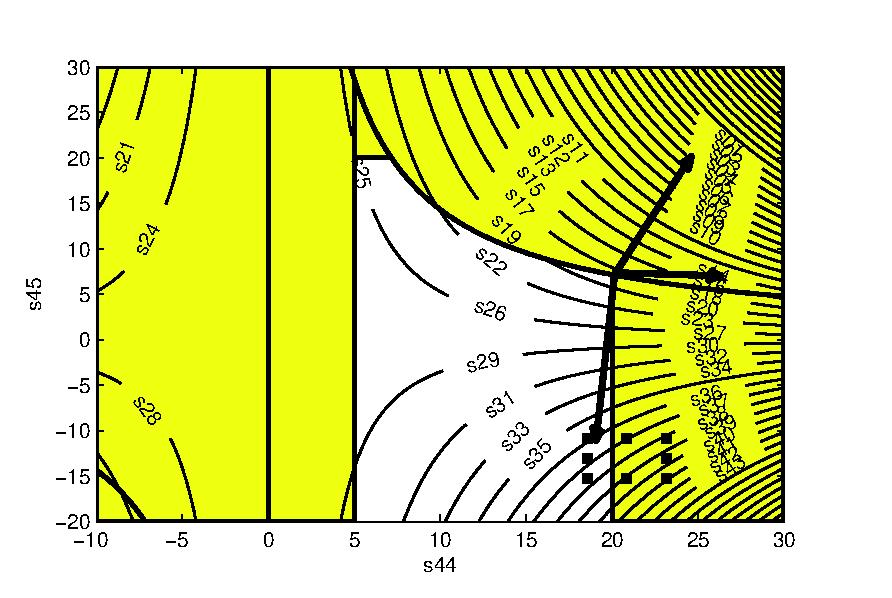
\includegraphics{unnamed.eps}}%
\end{psfrags}%
%
% End unnamed.tex
\end{document}
% See http://www.mathworks.de/matlabcentral/fileexchange/loadFile.do?objectId=4638
% for recent versions of laprint.m.
%
% created by:           LaPrint version 3.16 (13.9.2004)
% created on:           28-Dec-2013 21:44:20
% eps bounding box:     15 cm x 9.4415 cm
% comment:              
%
\begin{psfrags}%
\psfragscanon%
%
% text strings:
\psfrag{s01}[][]{\color[rgb]{0,0,0}\setlength{\tabcolsep}{0pt}\begin{tabular}{c}-48787.0859\end{tabular}}%
\psfrag{s02}[][]{\color[rgb]{0,0,0}\setlength{\tabcolsep}{0pt}\begin{tabular}{c}-46015.0924\end{tabular}}%
\psfrag{s03}[][]{\color[rgb]{0,0,0}\setlength{\tabcolsep}{0pt}\begin{tabular}{c}-43243.0989\end{tabular}}%
\psfrag{s04}[][]{\color[rgb]{0,0,0}\setlength{\tabcolsep}{0pt}\begin{tabular}{c}-40471.1054\end{tabular}}%
\psfrag{s05}[][]{\color[rgb]{0,0,0}\setlength{\tabcolsep}{0pt}\begin{tabular}{c}-37699.1118\end{tabular}}%
\psfrag{s06}[][]{\color[rgb]{0,0,0}\setlength{\tabcolsep}{0pt}\begin{tabular}{c}-34927.1183\end{tabular}}%
\psfrag{s07}[][]{\color[rgb]{0,0,0}\setlength{\tabcolsep}{0pt}\begin{tabular}{c}-32155.1248\end{tabular}}%
\psfrag{s08}[][]{\color[rgb]{0,0,0}\setlength{\tabcolsep}{0pt}\begin{tabular}{c}-29383.1313\end{tabular}}%
\psfrag{s09}[][]{\color[rgb]{0,0,0}\setlength{\tabcolsep}{0pt}\begin{tabular}{c}-26611.1378\end{tabular}}%
\psfrag{s10}[][]{\color[rgb]{0,0,0}\setlength{\tabcolsep}{0pt}\begin{tabular}{c}-23839.1443\end{tabular}}%
\psfrag{s11}[][]{\color[rgb]{0,0,0}\setlength{\tabcolsep}{0pt}\begin{tabular}{c}-21067.1507\end{tabular}}%
\psfrag{s12}[][]{\color[rgb]{0,0,0}\setlength{\tabcolsep}{0pt}\begin{tabular}{c}-18295.1572\end{tabular}}%
\psfrag{s13}[][]{\color[rgb]{0,0,0}\setlength{\tabcolsep}{0pt}\begin{tabular}{c}-15523.1637\end{tabular}}%
\psfrag{s14}[][]{\color[rgb]{0,0,0}\setlength{\tabcolsep}{0pt}\begin{tabular}{c}-15523.1637\end{tabular}}%
\psfrag{s15}[][]{\color[rgb]{0,0,0}\setlength{\tabcolsep}{0pt}\begin{tabular}{c}-12751.1702\end{tabular}}%
\psfrag{s16}[][]{\color[rgb]{0,0,0}\setlength{\tabcolsep}{0pt}\begin{tabular}{c}-12751.1702\end{tabular}}%
\psfrag{s17}[][]{\color[rgb]{0,0,0}\setlength{\tabcolsep}{0pt}\begin{tabular}{c}-9979.17666\end{tabular}}%
\psfrag{s18}[][]{\color[rgb]{0,0,0}\setlength{\tabcolsep}{0pt}\begin{tabular}{c}-9979.17666\end{tabular}}%
\psfrag{s19}[][]{\color[rgb]{0,0,0}\setlength{\tabcolsep}{0pt}\begin{tabular}{c}-7207.18315\end{tabular}}%
\psfrag{s20}[][]{\color[rgb]{0,0,0}\setlength{\tabcolsep}{0pt}\begin{tabular}{c}-7207.18315\end{tabular}}%
\psfrag{s21}[][]{\color[rgb]{0,0,0}\setlength{\tabcolsep}{0pt}\begin{tabular}{c}-4435.18963\end{tabular}}%
\psfrag{s22}[][]{\color[rgb]{0,0,0}\setlength{\tabcolsep}{0pt}\begin{tabular}{c}-4435.18963\end{tabular}}%
\psfrag{s23}[][]{\color[rgb]{0,0,0}\setlength{\tabcolsep}{0pt}\begin{tabular}{c}-4435.18963\end{tabular}}%
\psfrag{s24}[][]{\color[rgb]{0,0,0}\setlength{\tabcolsep}{0pt}\begin{tabular}{c}-1663.19611\end{tabular}}%
\psfrag{s25}[][]{\color[rgb]{0,0,0}\setlength{\tabcolsep}{0pt}\begin{tabular}{c}-1663.19611\end{tabular}}%
\psfrag{s26}[][]{\color[rgb]{0,0,0}\setlength{\tabcolsep}{0pt}\begin{tabular}{c}-1663.19611\end{tabular}}%
\psfrag{s27}[][]{\color[rgb]{0,0,0}\setlength{\tabcolsep}{0pt}\begin{tabular}{c}-1663.19611\end{tabular}}%
\psfrag{s28}[][]{\color[rgb]{0,0,0}\setlength{\tabcolsep}{0pt}\begin{tabular}{c}1108.79741\end{tabular}}%
\psfrag{s29}[][]{\color[rgb]{0,0,0}\setlength{\tabcolsep}{0pt}\begin{tabular}{c}1108.79741\end{tabular}}%
\psfrag{s30}[][]{\color[rgb]{0,0,0}\setlength{\tabcolsep}{0pt}\begin{tabular}{c}1108.79741\end{tabular}}%
\psfrag{s31}[][]{\color[rgb]{0,0,0}\setlength{\tabcolsep}{0pt}\begin{tabular}{c}3880.79093\end{tabular}}%
\psfrag{s32}[][]{\color[rgb]{0,0,0}\setlength{\tabcolsep}{0pt}\begin{tabular}{c}3880.79093\end{tabular}}%
\psfrag{s33}[][]{\color[rgb]{0,0,0}\setlength{\tabcolsep}{0pt}\begin{tabular}{c}6652.78444\end{tabular}}%
\psfrag{s34}[][]{\color[rgb]{0,0,0}\setlength{\tabcolsep}{0pt}\begin{tabular}{c}6652.78444\end{tabular}}%
\psfrag{s35}[][]{\color[rgb]{0,0,0}\setlength{\tabcolsep}{0pt}\begin{tabular}{c}9424.77796\end{tabular}}%
\psfrag{s36}[][]{\color[rgb]{0,0,0}\setlength{\tabcolsep}{0pt}\begin{tabular}{c}12196.7715\end{tabular}}%
\psfrag{s37}[][]{\color[rgb]{0,0,0}\setlength{\tabcolsep}{0pt}\begin{tabular}{c}14968.765\end{tabular}}%
\psfrag{s38}[][]{\color[rgb]{0,0,0}\setlength{\tabcolsep}{0pt}\begin{tabular}{c}17740.7585\end{tabular}}%
\psfrag{s39}[][]{\color[rgb]{0,0,0}\setlength{\tabcolsep}{0pt}\begin{tabular}{c}20512.752\end{tabular}}%
\psfrag{s40}[][]{\color[rgb]{0,0,0}\setlength{\tabcolsep}{0pt}\begin{tabular}{c}23284.7456\end{tabular}}%
\psfrag{s41}[][]{\color[rgb]{0,0,0}\setlength{\tabcolsep}{0pt}\begin{tabular}{c}26056.7391\end{tabular}}%
\psfrag{s42}[][]{\color[rgb]{0,0,0}\setlength{\tabcolsep}{0pt}\begin{tabular}{c}28828.7326\end{tabular}}%
\psfrag{s43}[][]{\color[rgb]{0,0,0}\setlength{\tabcolsep}{0pt}\begin{tabular}{c}31600.7261\end{tabular}}%
\psfrag{s44}[t][t]{\color[rgb]{0,0,0}\setlength{\tabcolsep}{0pt}\begin{tabular}{c}x\end{tabular}}%
\psfrag{s45}[b][b]{\color[rgb]{0,0,0}\setlength{\tabcolsep}{0pt}\begin{tabular}{c}y\end{tabular}}%
\psfrag{s52}[lt][lt]{\color[rgb]{0,0,0}\setlength{\tabcolsep}{0pt}\begin{tabular}{l}g_1\end{tabular}}%
\psfrag{s53}[lt][lt]{\color[rgb]{0,0,0}\setlength{\tabcolsep}{0pt}\begin{tabular}{l}g_5\end{tabular}}%
\psfrag{s54}[lt][lt]{\color[rgb]{0,0,0}\setlength{\tabcolsep}{0pt}\begin{tabular}{l}f\end{tabular}}%
%
% Figure:
\resizebox{12cm}{!}{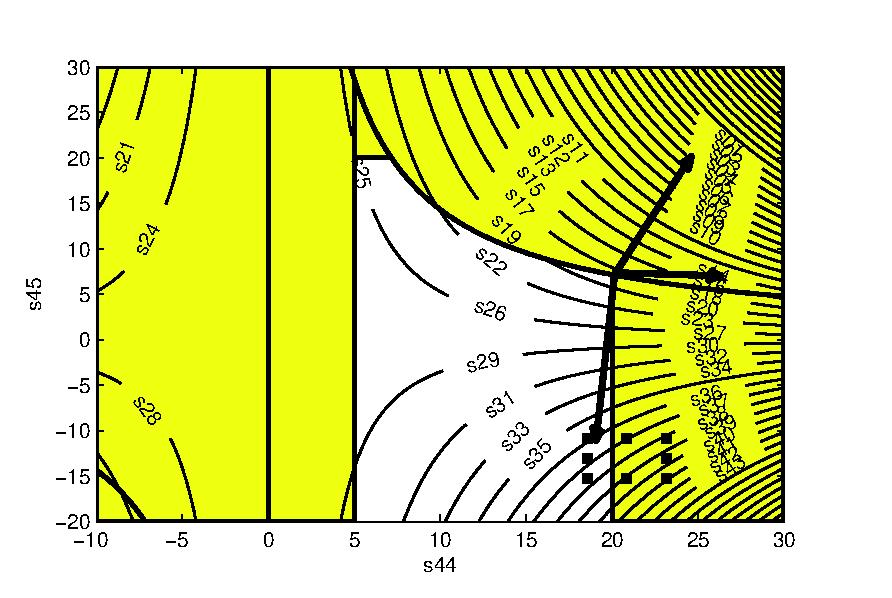
\includegraphics{unnamed.eps}}%
\end{psfrags}%
%
% End unnamed.tex
